% Options for packages loaded elsewhere
\PassOptionsToPackage{unicode}{hyperref}
\PassOptionsToPackage{hyphens}{url}
%
\documentclass[
  man,floatsintext]{apa6}
\usepackage{amsmath,amssymb}
\usepackage{iftex}
\ifPDFTeX
  \usepackage[T1]{fontenc}
  \usepackage[utf8]{inputenc}
  \usepackage{textcomp} % provide euro and other symbols
\else % if luatex or xetex
  \usepackage{unicode-math} % this also loads fontspec
  \defaultfontfeatures{Scale=MatchLowercase}
  \defaultfontfeatures[\rmfamily]{Ligatures=TeX,Scale=1}
\fi
\usepackage{lmodern}
\ifPDFTeX\else
  % xetex/luatex font selection
\fi
% Use upquote if available, for straight quotes in verbatim environments
\IfFileExists{upquote.sty}{\usepackage{upquote}}{}
\IfFileExists{microtype.sty}{% use microtype if available
  \usepackage[]{microtype}
  \UseMicrotypeSet[protrusion]{basicmath} % disable protrusion for tt fonts
}{}
\makeatletter
\@ifundefined{KOMAClassName}{% if non-KOMA class
  \IfFileExists{parskip.sty}{%
    \usepackage{parskip}
  }{% else
    \setlength{\parindent}{0pt}
    \setlength{\parskip}{6pt plus 2pt minus 1pt}}
}{% if KOMA class
  \KOMAoptions{parskip=half}}
\makeatother
\usepackage{xcolor}
\usepackage{graphicx}
\makeatletter
\def\maxwidth{\ifdim\Gin@nat@width>\linewidth\linewidth\else\Gin@nat@width\fi}
\def\maxheight{\ifdim\Gin@nat@height>\textheight\textheight\else\Gin@nat@height\fi}
\makeatother
% Scale images if necessary, so that they will not overflow the page
% margins by default, and it is still possible to overwrite the defaults
% using explicit options in \includegraphics[width, height, ...]{}
\setkeys{Gin}{width=\maxwidth,height=\maxheight,keepaspectratio}
% Set default figure placement to htbp
\makeatletter
\def\fps@figure{htbp}
\makeatother
\setlength{\emergencystretch}{3em} % prevent overfull lines
\providecommand{\tightlist}{%
  \setlength{\itemsep}{0pt}\setlength{\parskip}{0pt}}
\setcounter{secnumdepth}{-\maxdimen} % remove section numbering
% Make \paragraph and \subparagraph free-standing
\ifx\paragraph\undefined\else
  \let\oldparagraph\paragraph
  \renewcommand{\paragraph}[1]{\oldparagraph{#1}\mbox{}}
\fi
\ifx\subparagraph\undefined\else
  \let\oldsubparagraph\subparagraph
  \renewcommand{\subparagraph}[1]{\oldsubparagraph{#1}\mbox{}}
\fi
% definitions for citeproc citations
\NewDocumentCommand\citeproctext{}{}
\NewDocumentCommand\citeproc{mm}{%
  \begingroup\def\citeproctext{#2}\cite{#1}\endgroup}
\makeatletter
 % allow citations to break across lines
 \let\@cite@ofmt\@firstofone
 % avoid brackets around text for \cite:
 \def\@biblabel#1{}
 \def\@cite#1#2{{#1\if@tempswa , #2\fi}}
\makeatother
\newlength{\cslhangindent}
\setlength{\cslhangindent}{1.5em}
\newlength{\csllabelwidth}
\setlength{\csllabelwidth}{3em}
\newenvironment{CSLReferences}[2] % #1 hanging-indent, #2 entry-spacing
 {\begin{list}{}{%
  \setlength{\itemindent}{0pt}
  \setlength{\leftmargin}{0pt}
  \setlength{\parsep}{0pt}
  % turn on hanging indent if param 1 is 1
  \ifodd #1
   \setlength{\leftmargin}{\cslhangindent}
   \setlength{\itemindent}{-1\cslhangindent}
  \fi
  % set entry spacing
  \setlength{\itemsep}{#2\baselineskip}}}
 {\end{list}}
\usepackage{calc}
\newcommand{\CSLBlock}[1]{\hfill\break\parbox[t]{\linewidth}{\strut\ignorespaces#1\strut}}
\newcommand{\CSLLeftMargin}[1]{\parbox[t]{\csllabelwidth}{\strut#1\strut}}
\newcommand{\CSLRightInline}[1]{\parbox[t]{\linewidth - \csllabelwidth}{\strut#1\strut}}
\newcommand{\CSLIndent}[1]{\hspace{\cslhangindent}#1}
\ifLuaTeX
\usepackage[bidi=basic]{babel}
\else
\usepackage[bidi=default]{babel}
\fi
\babelprovide[main,import]{english}
% get rid of language-specific shorthands (see #6817):
\let\LanguageShortHands\languageshorthands
\def\languageshorthands#1{}
% Manuscript styling
\usepackage{upgreek}
\captionsetup{font=singlespacing,justification=justified}

% Table formatting
\usepackage{longtable}
\usepackage{lscape}
% \usepackage[counterclockwise]{rotating}   % Landscape page setup for large tables
\usepackage{multirow}		% Table styling
\usepackage{tabularx}		% Control Column width
\usepackage[flushleft]{threeparttable}	% Allows for three part tables with a specified notes section
\usepackage{threeparttablex}            % Lets threeparttable work with longtable

% Create new environments so endfloat can handle them
% \newenvironment{ltable}
%   {\begin{landscape}\centering\begin{threeparttable}}
%   {\end{threeparttable}\end{landscape}}
\newenvironment{lltable}{\begin{landscape}\centering\begin{ThreePartTable}}{\end{ThreePartTable}\end{landscape}}

% Enables adjusting longtable caption width to table width
% Solution found at http://golatex.de/longtable-mit-caption-so-breit-wie-die-tabelle-t15767.html
\makeatletter
\newcommand\LastLTentrywidth{1em}
\newlength\longtablewidth
\setlength{\longtablewidth}{1in}
\newcommand{\getlongtablewidth}{\begingroup \ifcsname LT@\roman{LT@tables}\endcsname \global\longtablewidth=0pt \renewcommand{\LT@entry}[2]{\global\advance\longtablewidth by ##2\relax\gdef\LastLTentrywidth{##2}}\@nameuse{LT@\roman{LT@tables}} \fi \endgroup}

% \setlength{\parindent}{0.5in}
% \setlength{\parskip}{0pt plus 0pt minus 0pt}

% Overwrite redefinition of paragraph and subparagraph by the default LaTeX template
% See https://github.com/crsh/papaja/issues/292
\makeatletter
\renewcommand{\paragraph}{\@startsection{paragraph}{4}{\parindent}%
  {0\baselineskip \@plus 0.2ex \@minus 0.2ex}%
  {-1em}%
  {\normalfont\normalsize\bfseries\itshape\typesectitle}}

\renewcommand{\subparagraph}[1]{\@startsection{subparagraph}{5}{1em}%
  {0\baselineskip \@plus 0.2ex \@minus 0.2ex}%
  {-\z@\relax}%
  {\normalfont\normalsize\itshape\hspace{\parindent}{#1}\textit{\addperi}}{\relax}}
\makeatother

\makeatletter
\usepackage{etoolbox}
\patchcmd{\maketitle}
  {\section{\normalfont\normalsize\abstractname}}
  {\section*{\normalfont\normalsize\abstractname}}
  {}{\typeout{Failed to patch abstract.}}
\patchcmd{\maketitle}
  {\section{\protect\normalfont{\@title}}}
  {\section*{\protect\normalfont{\@title}}}
  {}{\typeout{Failed to patch title.}}
\makeatother

\usepackage{xpatch}
\makeatletter
\xapptocmd\appendix
  {\xapptocmd\section
    {\addcontentsline{toc}{section}{\appendixname\ifoneappendix\else~\theappendix\fi: #1}}
    {}{\InnerPatchFailed}%
  }
{}{\PatchFailed}
\makeatother
\keywords{keywords\newline\indent Word count: X}
\usepackage{lineno}

\linenumbers
\usepackage{csquotes}
\ifLuaTeX
  \usepackage{selnolig}  % disable illegal ligatures
\fi
\usepackage{bookmark}
\IfFileExists{xurl.sty}{\usepackage{xurl}}{} % add URL line breaks if available
\urlstyle{same}
\hypersetup{
  pdftitle={Proportional Reasoning Across Formats},
  pdfauthor={Maanav Choudhary1},
  pdflang={en-EN},
  pdfkeywords={keywords},
  hidelinks,
  pdfcreator={LaTeX via pandoc}}

\title{Proportional Reasoning Across Formats}
\author{Maanav Choudhary\textsuperscript{1}}
\date{}


\shorttitle{Proportional Reasoning}

\authornote{

This is Maanav's Assignment 11, it was fun and challenging!

The authors made the following contributions. Maanav Choudhary: Conceptualization, Writing - Original Draft Preparation, Writing - Review \& Editing.

Correspondence concerning this article should be addressed to Maanav Choudhary, N/A. E-mail: \href{mailto:maanavpilania63@gmail.com}{\nolinkurl{maanavpilania63@gmail.com}}

}

\affiliation{\vspace{0.5cm}\textsuperscript{1} Rutgers University}

\abstract{%
Comparing proportions is a fundamental skill that even infants seem to possess, albeit at a rudimentary level. This study explores how well people compare proportions when presented in different visual formats, aiming to deepen our understanding of this cognitive process. Specifically, we examined whether average performance varies across format types, whether numerator congruency status influences performance, and whether an interaction exists between format type and numerator congruency. Here, we show that both format type and numerator congruency significantly impact performance, with notable interactions between these factors. These findings reveal that certain formats and congruency conditions facilitate more accurate comparisons, advancing previous knowledge by highlighting the importance of presentation design in proportion reasoning. This work contributes to a broader understanding of cognitive processing in numerical tasks and has implications for designing more effective educational and communicative tools.
}



\begin{document}
\maketitle

\section{Methods}\label{methods}

Here we outline how the data was collected, as well as information on the participants and materials used.

\subsection{Participants}\label{participants}

A total of 99 adults participated in this study.

\subsection{Material}\label{material}

The images provided to the participants had a mix of blue and orange. Some images had these represented as blobs, and some as dots. There were four conditions for the mix of blue and orange.

\begin{figure}
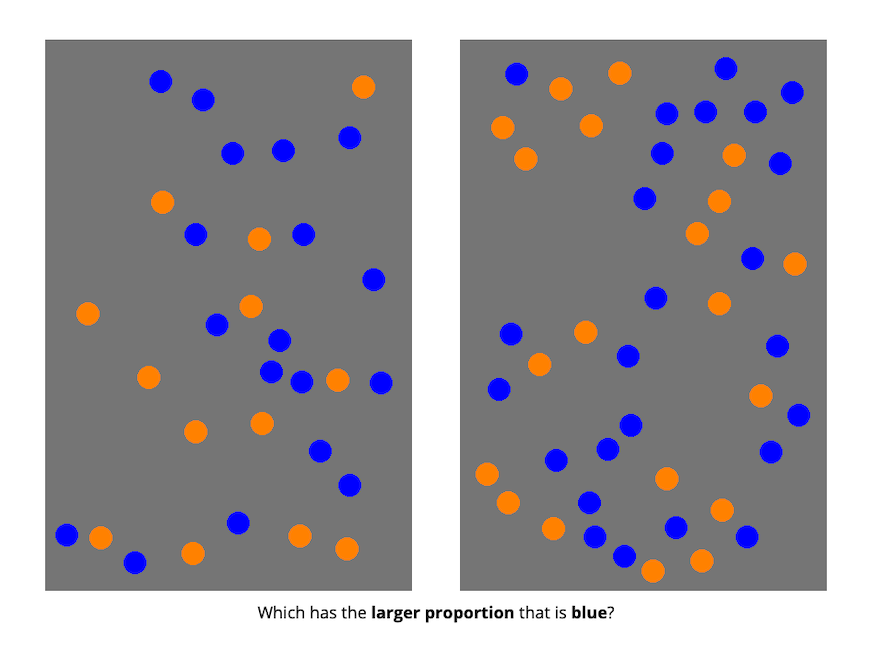
\includegraphics[width=2.98in]{images_WA10/Probtask_Trial} \caption{Example of an image given to participants.}\label{fig:example-img}
\end{figure}

\subsection{Procedure}\label{procedure}

First, participants were introduced to a story about a magic ball and that the outcome (i.e., blue or orange) depended on the proportions. Then they were asked to compare the proportions of different images, for example the ones shown in Figure \ref{fig:example-img}

In other words, participants were shown to images of the same kind at the same time and asked to decide which had a higher proportion of the shape (or dots) colored in blue.

\subsection{Data analysis}\label{data-analysis}

We used R (Version 4.4.1; R Core Team, 2024) and the R-packages \emph{dplyr} (Version 1.1.4; Wickham, François, Henry, Müller, \& Vaughan, 2023), \emph{ggdist} (Version 3.3.2; Kay, 2024), \emph{ggplot2} (Version 3.5.1; Wickham, 2016), \emph{papaja} (Version 0.1.3; Aust \& Barth, 2024), \emph{tibble} (Version 3.2.1; Müller \& Wickham, 2023), \emph{tidyr} (Version 1.3.1; Wickham, Vaughan, \& Girlich, 2024) and \emph{tidyverse} (Version 2.0.0; Wickham et al., 2019) for all our analyses.

\newpage

\section{Results}\label{results}

\begin{enumerate}
\def\labelenumi{\arabic{enumi}.}
\tightlist
\item
  Does average performance vary across format types, ignoring all other aspects of the stimuli?
\end{enumerate}

\begin{figure}
\centering
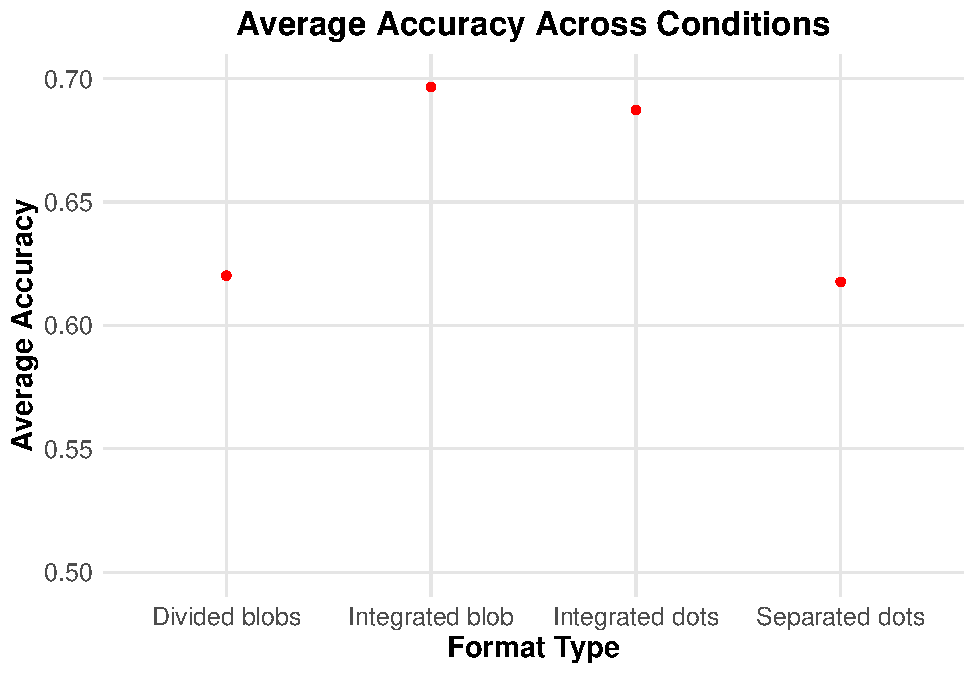
\includegraphics{Choudhary_WA11_files/figure-latex/performance-plot-1.pdf}
\caption{\label{fig:performance-plot}Average Performance.}
\end{figure}

Figure \ref{fig:performance-plot} shows the average accuracry for all format types, showing that the integrated blobs and integrated dots both showed a higher average than the separated blobs and dots, the averages of the priors being close to each other(.01 apart) and the averages of the latter being close to each other (.003 apart)

\begin{enumerate}
\def\labelenumi{\arabic{enumi}.}
\setcounter{enumi}{1}
\tightlist
\item
  How are reaction time and accuracy related?
  \newpage
\end{enumerate}

\begin{figure}
\centering
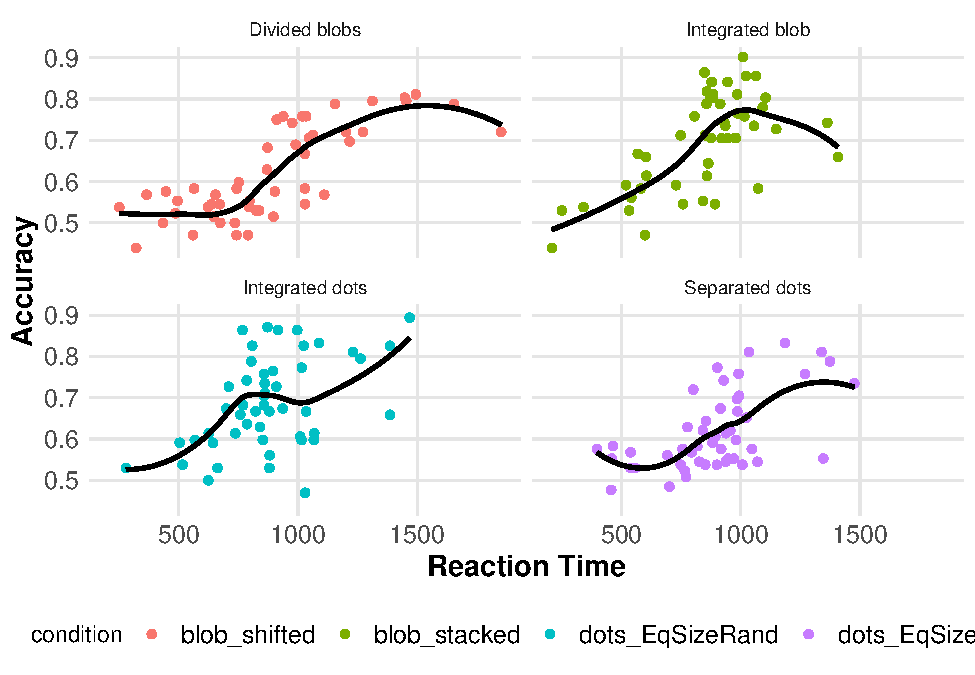
\includegraphics{Choudhary_WA11_files/figure-latex/rt-1.pdf}
\caption{\label{fig:rt}Reaction Time}
\end{figure}

Figure \ref{fig:rt} outlines that across all format types, as the reaction time becomes longer, accuracy rises. The lines of best fit show that in most conditions this increase drops off after a certain point.

\newpage

\begin{enumerate}
\def\labelenumi{\arabic{enumi}.}
\setcounter{enumi}{2}
\tightlist
\item
  How does numerator congruency interact with format type?
\end{enumerate}

\begin{figure}
\centering
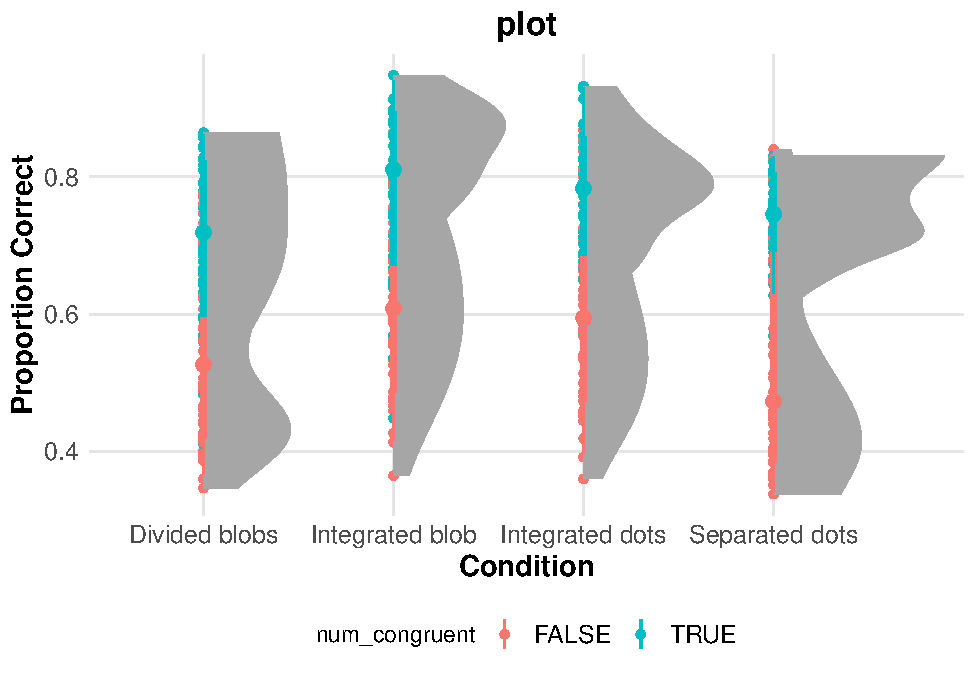
\includegraphics{Choudhary_WA11_files/figure-latex/num-con-1.pdf}
\caption{\label{fig:num-con}Numerator Congruency and Correctness}
\end{figure}

The figure \ref{fig:num-con} above shows that, for all conditions, when the numerators are congruent the proportion of correct responses is higher.

\section{Discussion}\label{discussion}

\subsection{Interpretation}\label{interpretation}

\begin{enumerate}
\def\labelenumi{\arabic{enumi}.}
\tightlist
\item
  Does average performance vary across format type?
\end{enumerate}

The data shows that the average performance does indeed vary across format type. The data indicates that when blobs and dots are integrated, the performance is higher than when they are separated. The performance difference between blobs and dots when they are both separated or integrated is not very large (.68 and .69 for integrated and .617 and .62 for separated). The higher averages for integrated data vs separated that this data shows indicates that humans may deal better with integrated visuals than separated when gauging quantity.

\begin{enumerate}
\def\labelenumi{\arabic{enumi}.}
\setcounter{enumi}{1}
\tightlist
\item
  Does average performance vary across numerator congruency status?
\end{enumerate}

The average performance is higher on when the numerators are congruent then when they are not.

\begin{enumerate}
\def\labelenumi{\arabic{enumi}.}
\setcounter{enumi}{2}
\tightlist
\item
  Does numerator congruency vary across format type? (i.e., is there an interaction)
\end{enumerate}

Numerator concurrency seems vary slightly across format type. Both of the dot cases appear to have less numerator concurrency than the blob conditions.

\subsection{Conclusion}\label{conclusion}

\begin{enumerate}
\def\labelenumi{\arabic{enumi}.}
\item
  One of the hardest parts of the assignment was interpreting how the data and graphs related to the research objectives, and trying to turn the visual information into something written and coherent.
\item
  The most satisfying and enjoyable part of the assignment was figuring out how to insert the images, and playing around with the format to make it visually appealing.
\end{enumerate}

\newpage

\section{References}\label{references}

\phantomsection\label{refs}
\begin{CSLReferences}{1}{0}
\bibitem[\citeproctext]{ref-R-papaja}
Aust, F., \& Barth, M. (2024). \emph{{papaja}: {Prepare} reproducible {APA} journal articles with {R Markdown}}. \url{https://doi.org/10.32614/CRAN.package.papaja}

\bibitem[\citeproctext]{ref-R-ggdist}
Kay, M. (2024). {ggdist}: Visualizations of distributions and uncertainty in the grammar of graphics. \emph{IEEE Transactions on Visualization and Computer Graphics}, \emph{30}(1), 414--424. \url{https://doi.org/10.1109/TVCG.2023.3327195}

\bibitem[\citeproctext]{ref-R-tibble}
Müller, K., \& Wickham, H. (2023). \emph{Tibble: Simple data frames}. Retrieved from \url{https://CRAN.R-project.org/package=tibble}

\bibitem[\citeproctext]{ref-R-base}
R Core Team. (2024). \emph{R: A language and environment for statistical computing}. Vienna, Austria: R Foundation for Statistical Computing. Retrieved from \url{https://www.R-project.org/}

\bibitem[\citeproctext]{ref-R-ggplot2}
Wickham, H. (2016). \emph{ggplot2: Elegant graphics for data analysis}. Springer-Verlag New York. Retrieved from \url{https://ggplot2.tidyverse.org}

\bibitem[\citeproctext]{ref-R-tidyverse}
Wickham, H., Averick, M., Bryan, J., Chang, W., McGowan, L. D., François, R., \ldots{} Yutani, H. (2019). Welcome to the {tidyverse}. \emph{Journal of Open Source Software}, \emph{4}(43), 1686. \url{https://doi.org/10.21105/joss.01686}

\bibitem[\citeproctext]{ref-R-dplyr}
Wickham, H., François, R., Henry, L., Müller, K., \& Vaughan, D. (2023). \emph{Dplyr: A grammar of data manipulation}. Retrieved from \url{https://CRAN.R-project.org/package=dplyr}

\bibitem[\citeproctext]{ref-R-tidyr}
Wickham, H., Vaughan, D., \& Girlich, M. (2024). \emph{Tidyr: Tidy messy data}. Retrieved from \url{https://CRAN.R-project.org/package=tidyr}

\end{CSLReferences}


\end{document}
